\documentclass[10pt, a4paper,openany]{article}
\usepackage[italian]{babel}
\usepackage[T1]{fontenc}
\usepackage[table]{xcolor}
\usepackage{float}
\restylefloat{table,figure}
\usepackage{graphicx}	
\usepackage[utf8]{inputenc}
\usepackage{amsmath}
\usepackage{fancyhdr}
\usepackage{geometry}
\geometry{a4paper,top=2cm,bottom=2cm,left=2.5cm,right=2.5cm,%
	    heightrounded,bindingoffset=5mm}
\usepackage{amssymb}
\usepackage{amsthm}
\usepackage{multicol}
\usepackage{xcolor}
\usepackage{hyperref}
\usepackage{caption}
%\usepackage{url}
%inizia qui aggiunta
\usepackage{collcell}
\usepackage{hhline}
\usepackage{pgf}
\usepackage{multirow}
\usepackage{fancyvrb}
\usepackage{verbatim}


\begin{document}
\begin{center}
\large\textbf{Guida operativa}
\end{center}

\begin{center}
 Federico Luzzi,  Marco Peracchi, Christian Uccheddu, Gabriele Centemeri (TTC)
\end{center}
Di seguito la guida operativa per eseguire il codice in modo da replicare i risultati ottenuti:

\section*{Presa dati Dicembre}

Eseguire il file:

\begin{verbatim}
scraper/scraper_csv.py
\end{verbatim}
Questo script serve ad effettuare una rilevazione dati ogni 6h. I dati così estratti vengono trasformati in csv.
Trasformare i dati da csv in json usando: 

\begin{verbatim}
csv_to_json/main.py
\end{verbatim}
Per eseguire lo script è necessario fornire il seguente parametro:
\begin{itemize}
	\item -d "directory\_dei\_dati"
\end{itemize}
Caricare quindi i json su mongo usando: 

\begin{verbatim}
json_to_mongo/json_to_mongo.py
\end{verbatim}
A questo script vanno forniti i seguenti parametri:

\begin{itemize}
	\item -d "directory dei dati"
	\item -u "utente mongo"
	\item -p "password utente"
	\item -port "porta in cui è attivo l'utente"
	\item-db "Nome del database in output"
	\item -c "collection in cui vengono inseriti i dati"
\end{itemize}

\section*{Presa dati periodo Covid}

Aprire il servizio mongo da terminale.


Lanciare in due terminali contemporaneamente: 

\begin{itemize}
	\item \begin{verbatim}
	scraper/scraper_consumer.py
	\end{verbatim}
	\item \begin{verbatim}
scraper/scraper_producer.py
	\end{verbatim}
\end{itemize}

Questo effettua una rilevazione dati ogni 6h attraverso il servizio kafka. L'utilizzo di kafka non è indispensabile, inizialmente però avevamo deciso di prendere i dati sia dei canali che dei video in live stream quindi kafka aveva senso in quanto venivano usati due topic diversi e fatte le prime operazioni preliminari. Abbiamo deciso di tenerlo per non stravolgere la pipeline di esecuzione.

\section*{Presa dati Covid}

Scaricare i dati in formato csv da \href{https://ourworldindata.org/coronavirus-testing}{questo sito}
\\Eseguire il codice:

\begin{verbatim}
covid/cleaner.py
\end{verbatim}
Questo script permette di eseguire una pulizia dei dati in modo da renderli integrabili con i json raccolti in precedenza.


\section*{Integrazione dei dati}


Per eseguire l'integrazione tra i dati covid e i dati di youtube bisogna eseguire il seguente script:

\begin{verbatim}
clean_store_data/merge_to_mongo.py
\end{verbatim}
A questo script vanno forniti i seguenti parametri:

\begin{itemize}
	\item -d "directory dei dati"
	\item -u "utente mongo"
	\item -p "password utente"
	\item -port "porta in cui è attivo l'utente"
	\item-db "Nome del database in output"
	\item -c "collection in cui vengono inseriti i dati"
\end{itemize}
Questo script integra i due dataset e carica tutto su mongo.


\section*{Query mongo}


Per le visualizzazioni che intendiamo fare abbiamo bisogno di poter distinguere quando un video contenga nel titolo o nei tag una delle parole che si rifanno al coronavirus. Per controllare questo è stata costruita la seguente espressione regolare:

\begin{figure}[H]
	\centering
	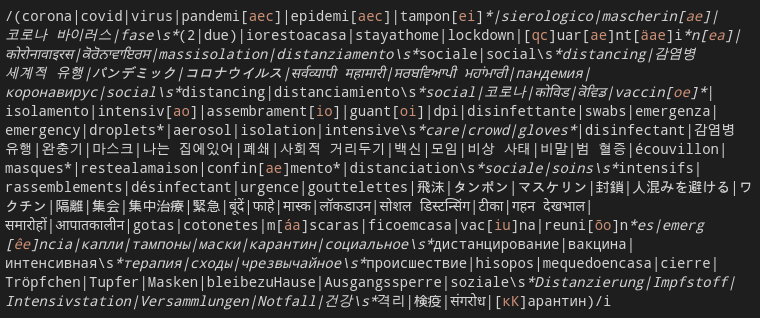
\includegraphics[height=0.4 \linewidth]{rexpression.png}
	\caption{Regular expression usata}
\end{figure}



Creare due nuovi campi chiamati \textbf{covid\_title} e \textbf{covid\_tags} settati entrambi a \textbf{False} 

\begin{Verbatim}[frame=single,baselinestretch=0.1]
db.video_merge.update({},{$set : {covid_tags : false, 
			covid_title : false}},
			{multi : true})
\end{Verbatim}
Eseguire le seguenti due query che controllano se l'espressione regolare è presente nel campo title o in uno dei tag per ogni video.

\begin{Verbatim}[frame=single,baselinestretch=0.1]
db.video_merge.update({tags : {$in : [REGEX]}}, 
			{$set : {covid_tags: true}}, 
			{multi : true})
\end{Verbatim}
 \begin{Verbatim}[frame=single,baselinestretch=0.1]
db.video_merge.update({title : {$in : [REGEX]}}, 
			{$set : {covid_title: true}}, 
			{multi : true})
\end{Verbatim}


\end{document}


